\documentclass[11pt]{article}
\usepackage[margin = 1in]{geometry}
\usepackage{amsmath}
\usepackage{amssymb}
\usepackage{amsthm}
\usepackage{graphicx}
\usepackage{enumitem}
\usepackage{url}
\usepackage[parfill]{parskip}
\usepackage{listings}
\newcommand{\skipline}{\vspace{\baselineskip}}
\newcommand{\spacer}{\noalign{\medskip}}
\newcommand{~}{\sim}
\newenvironment{problem}[1]{\textbf{Problem #1: }}{\newpage}
\usepackage{caption}
\usepackage{subcaption}
\usepackage[utf8]{inputenc}
\usepackage{xcolor}
\definecolor{codegreen}{rgb}{0,0.6,0}
\definecolor{codegray}{rgb}{0.5,0.5,0.5}
\definecolor{codepurple}{rgb}{0.58,0,0.82}
\definecolor{backcolour}{rgb}{0.95,0.95,0.92}
\lstdefinestyle{mystyle}{
	backgroundcolor=\color{backcolour},   
	commentstyle=\color{codegreen},
	keywordstyle=\color{magenta},
	numberstyle=\tiny\color{codegray},
	stringstyle=\color{codepurple},
	basicstyle=\ttfamily\footnotesize,
	breakatwhitespace=false,         
	breaklines=true,                 
	captionpos=b,                    
	keepspaces=true,                 
	numbers=left,                    
	numbersep=5pt,                  
	showspaces=false,                
	showstringspaces=false,
	showtabs=false,                  
	tabsize=2
}
\lstset{style=mystyle}

\begin{document}
	
	\begin{center}
		\textbf{Final Part B} \\
		\textbf{Ordinary Differential Equations} \\
		\textbf{Math 537} \\
		\textbf{Stephen Giang RedID: 823184070} \\
		\skipline \skipline
	\end{center}

	\begin{problem}{1 [ 8:40am, 8:53am]}
		 Consider the following 2nd order ODEs:
		 \[\frac{d^2X}{dt^2} - a^2X = F(t) \tag{1.1}\]
		 \[\frac{d^2X}{dt^2} + a^2X = F(t) \tag{1.2}\]
		 Complete the following problems:
		 \begin{enumerate}[label = (\alph*)]
		 	\item Assume that $F = G = 0$ and $a$ is a positive constant. Solve	Eqs. (1.1) and (1.2) for general solutions
		 	\\ \\
		 	Notice the characteristic equation for Eq (1.1):
		 	\[\lambda^2 - a^2 = 0, \qquad \lambda = \pm {a}\]
		 	Thus from these eigenvalues, we get the following solution:
		 	\[X = c_1e^{-{a}} + c_2e^{{a}}\]
		 	Notice the characteristic equation for Eq (1.2):
		 	\[\lambda^2 + a^2 = 0, \qquad \lambda = \pm i{a}\]
		 	Thus from these eigenvalues, we get the following solution:
		 	\[X = c_1\left(\cos({a}t) + i\sin({a}t)\right) \]
		 	\item Find $F(t)$ so that Eq. (1.1) has repeated eigenvalue. Briefly
		 	discuss the characteristics of the particular solution. [$a$ is a positive constant.]
		 	\item Find $G(t)$ so that Eq. (1.1) has repeated eigenvalue. Briefly
		 	discuss the characteristics of the particular solution. [$a$ is a positive constant.]
		 	\item  State the conditions under which the solutions in problem (1a)
		 	change rapidly within an interval or oscillate rapidly over a global scale.
		 	\item  Assume $F = G = 0$ and $a(t) > 0$ is a function of time. Briefly
		 	discuss how to solve both systems.
		 \end{enumerate}
	\end{problem}
	
	\begin{problem}{2 [ 9:47am, 9:57am]}
		Consider the following 2nd order ODE for nonlinear pendulum
		oscillations (as shown in Figure 1):
		\[\frac{d^2\theta}{dt^2} + \epsilon\frac{d\theta}{dt} + \sin\theta = 0\tag{2.1}\]
		Apply the full equation and its simplified versions to discuss the following
		concepts:
		\begin{enumerate}[label = (\alph*)]
			\item Locally linearized systems near a stable or unstable critical
			point.
			\item The impact of dissipation on the local, global, and structural
			stability.

			\item The impact of nonlinearity (e.g., represented by a cubic term)
			on the local, global, and structural stability.

			\[\frac{d^2z}{dt^2} + \theta = 0. \tag{2.2}\]
			\[\frac{d^2z}{dt^2} + \epsilon \frac{dz}{dt} + \theta = 0. \tag{2.3}\]
			\[\frac{d^2z}{dt^2} + \left(\theta - \frac{\theta^3}{6}\right) = 0. \tag{2.4}\]
			\begin{itemize}
				\item[(2.2) ] We can find the eigenvalues from solving its characteristic equation.
				\[\lambda^2 + 1 = 0\]
				Thus our eigenvalues are $\lambda = \pm i$.  This means that we get a \textbf{Clockwise Center}.
				\item[(2.3) ] We can find the eigenvalues from solving its characteristic equation.
				\[\lambda^2 + \epsilon\lambda + 1 = 0\]
				Thus our eigenvalues are $\lambda = \frac{1}{2}\left(-\epsilon \pm \sqrt{\epsilon^2 - 4}\right)$.
				\\ \\
				For $\epsilon < -2$, we get 2 positive real eigenvalues.  This means that we get an \textbf{Unstable Source}.
				\\ \\
				For $\epsilon = - 2$, we get $\lambda = 1$.  This means that we get an \textbf{Unstable Source}.
				\\ \\
				For $-2 < \epsilon < 0$, we get 2 imaginary eigenvalues with positive real parts.  This means that we get an \textbf{Unstable Spiral}.
				\\ \\
				For $\epsilon = 0$, we get $\lambda = \pm i$.  This means that we get a \textbf{Clockwise Center}.
				\\ \\
				For $0 < \epsilon < 2$, we get 2 imaginary eigenvalues with negative real parts.  This means that we get a \textbf{Stable Spiral}.
				\\ \\
				For $2 < \epsilon$, we get 2 negative real eigenvalues.  This means that we get a \textbf{Stable Sink}.
				\\ \\
				For $\epsilon = 2$, we get $\lambda = -1$.  This means that we get a \textbf{Stable Sink}. 
				\newpage 
				\item[(2.4) ] Let $\phi = \theta'$ and $\phi' = \theta\left(\frac{\theta^2}{6} - 1 \right)$.
				\[X' = \begin{pmatrix}
					\phi \\ \phi'
				\end{pmatrix} = \begin{pmatrix}
					0 & 1 \\ \frac{\theta^2}{6} - 1 & 0
				\end{pmatrix}\begin{pmatrix}
					\theta \\ \phi
				\end{pmatrix} = AX\]
				Notice we can find the critical points:
				\[X' = \begin{pmatrix}
					0 \\ 0
				\end{pmatrix} = \begin{pmatrix}
					0 & 1 \\ \frac{\theta^2}{6} - 1 & 0
				\end{pmatrix}\begin{pmatrix}
					\theta \\ \phi
				\end{pmatrix} = AX\]
				From this we get the following critical points: $(\theta, \phi) = (\pm \sqrt{6},0)$ and $(\theta, \phi) = (0,0)$.
				\\ \\
				Now notice the Jacobian:
				\[J(\theta, \phi) = \left[\begin{array}{cc}
					\frac{d\phi}{d\theta} & \frac{d\phi}{d\theta'} \\
					\spacer \frac{d\phi'}{d\theta} & \frac{d\phi'}{d\theta'}	
				\end{array}\right] = \left[\begin{array}{cc}
					0 & 1 \\ \spacer \frac{\theta^2}{2} - 1 & 0
				\end{array}\right]\]
				Notice the Jacobians and eigenvalues evaluated at the critical points:
				\[J(0,0) = \begin{bmatrix}
					0 & 1 \\ -1 & 0
				\end{bmatrix}\] 
				From solving $|A - \lambda I| = 0$, we get that $\lambda = \pm i$.  Thus we get a \textbf{Clockwise Center}.
				\[J(\pm \sqrt{6}, 0) = \begin{bmatrix}
					0 & 1 \\ 2 & 0
				\end{bmatrix}\]
				From solving $|A - \lambda I| = 0$, we get that $\lambda = \pm \sqrt{2}$.  Thus we get a \textbf{Saddle Point}. \\
			\end{itemize}
			We get that for each point in which we have a saddle point, we get local minima for potential energy, and for centers, we get local maxima for potential energy.
		\end{enumerate}
	\end{problem}

	\begin{problem}{3 [ 8:07am, 8:39am][9:30, 9:43am] }
		Consider the Lorenz model:
		\[\frac{dX}{dt} = -\sigma X + \sigma Y \tag{3.1} \]
		\[\frac{dY}{dt} = -XZ + rX - \alpha Y \tag{3.2}\]
		\[\frac{dZ}{dt} = XY - \beta Z \tag{3.3}\]
		\begin{enumerate}[label = (\alph*)]
			\item Briefly discuss methods for analyzing the above nonlinear
			system.
			\\ \\
			We can compute the Jacobian and then evaluate the critical points using the Jacobian.  Then we can get the eigenvalues, and solve for the general solution.
			\item Compute a Jacobian matrix to obtain a linearized system.
			\\ \\
			Let $f_1 = \frac{dX}{dt}$, $f_2 = \frac{dY}{dt}$, $f_3 = \frac{dZ}{dt}$.  Notice the following Jacobian:
			\[J(X,Y,Z) = \left[\begin{array}{ccc}
				\frac{\partial f_1}{\partial X} & \frac{\partial f_1}{\partial Y} & \frac{\partial f_1}{\partial Z} \\
				\spacer\frac{\partial f_2}{\partial X} & \frac{\partial f_2}{\partial Y} & \frac{\partial f_2}{\partial Z} \\
				\spacer\frac{\partial f_3}{\partial X} & \frac{\partial f_3}{\partial Y} & \frac{\partial f_3}{\partial Z} \\
			\end{array}\right] = \left[ \begin{array}{ccc}
				-\sigma & \sigma & 0 \\
				\spacer -Z + r & -\alpha & -X \\
				\spacer Y & X & -\beta
			\end{array}\right]\]
			\item Apply a perturbation method to obtain systems of equations
			for basic state $O(\epsilon^0)$ and perturbation $O(\epsilon^1)$ variables
			\\ \\
			Notice the perturbation steps:
			\[\frac{dX}{dt} + \epsilon\frac{d^2X}{dt} = -\sigma (X + \epsilon X') + \sigma (Y + \epsilon Y') \]
			\[\frac{dY}{dt} + \epsilon\frac{d^2Y}{dt}= -(X + \epsilon X')(Z + \epsilon Z') + r(X + \epsilon X') - \alpha (Y + \epsilon Y') \]
			\[\frac{dZ}{dt} + \epsilon\frac{d^2Z}{dt}= (X + \epsilon X')(Y + \epsilon Y') - \beta (Z + \epsilon Z')\]
			Now if we look at the basic state of $O(\epsilon^0)$, we get:
			\[\frac{dX}{dt} + \epsilon\frac{d^2X}{dt}   = -\sigma X + \sigma Y \]
			\[\frac{dY}{dt} + \epsilon\frac{d^2Y}{dt}  = -XZ + rX - \alpha Y \]
			\[\frac{dZ}{dt} + \epsilon\frac{d^2Z}{dt} = XY - \beta Z\]
			Now if we look at the basic state of $O(\epsilon^1)$, we get:
			\[\frac{dX}{dt} + \epsilon\frac{d^2X}{dt}   = -\sigma X' + \sigma Y' \]
			\[\frac{dY}{dt} + \epsilon\frac{d^2Y}{dt}  = X'Z + XZ'  + rX' - \alpha Y' \]
			\[\frac{dZ}{dt} + \epsilon\frac{d^2Z}{dt} = X'Y + XY' - \beta Z'\]
			\item Given $\sigma = 10$, $\alpha = 1$, $\beta = 8 / 3$, briefly discuss the
			characteristics of three types of solutions within different intervals of
			heating parameters $(r)$.
			\\ \\
			Notice the Jacobian, its critical points, and the Jacobian evaluated at these critical points, with the given values:
			\[J(X,Y,Z) = \left[ \begin{array}{ccc}
				-10 & 10 & 0 \\
				\spacer -Z + r & -1 & -X \\
				\spacer Y & X & -8/3
			\end{array}\right]\]
			We can find the critical points from the following:
			\[\left[\begin{array}{c}
				\frac{dX}{dt} \\ \spacer \frac{dY}{dt} \\ \spacer \frac{dZ}{dt}
			\end{array}\right] = \left[\begin{array}{c}
				0 \\ \spacer 0 \\ \spacer 0
			\end{array}\right] = \left[\begin{array}{ccc}
				-10 & 10 & 0 \\
				\spacer r & -1 & -X \\
				\spacer 0 & X & -8/3
			\end{array}\right]\left[\begin{array}{c}
				X \\ \spacer Y \\ Z
			\end{array}\right]\]
			We can see that we get the following critical point: $\boldsymbol{(0,0,0)}$.
			\\ \\
			Notice the Jacobian at the critical point:
			\[J(0,0,0) = \left[\begin{array}{ccc}
				-10 & 10 & 0 \\
				\spacer r & -1 & 0 \\
				\spacer 0 & 0 & -8/3
			\end{array}\right]\]
			Now we can find the characteristic equation by solving $|J - \lambda I| = 0$
			\begin{align*}
				(-10 - \lambda)(-1 - \lambda)(-8/3 - \lambda) - 10(r)(-8/3 - \lambda) &= 0 \\
				-{\lambda}^{3} -{\frac {41\,{\lambda}^{2}}{3}}-{\frac {118\,\lambda}{3}}-{\frac{80}{3}} + \frac{80r}{3} + 10\lambda &= 0 \\
				\lambda^3 + \frac {41\,{\lambda}^{2}}{3} + \frac{88\lambda}{3} + \frac{80}{3}(1 - r) = 0
			\end{align*}
			\item Find critical points for positive parameters.
			\item Find critical points within the non-dissipative system (ie, no $\sigma X$ in Eq (3.1) and $\alpha = \beta = 0$)
		\end{enumerate}
	\end{problem}

	\begin{problem}{5 [ 8:54am, 9:24am]}
		Consider a composite motion with the following harmonic
		oscillators:
		\[\frac{d^2x_1}{dt^2} = -\omega_1^2x_1, \tag{5.1} \]
		\[\frac{d^2x_2}{dt^2} = -\omega_2^2x_2, \tag{5.2} \]
		\begin{enumerate}[label = (\alph*)]
			\item Discuss the condition under which the composite motion with
			the two frequencies is periodic or quasi-periodic.
			\\ \\
			From this system, we get 2 solutions:
			\[x_1(t) = a_1\cos(\omega_1t) + b_1\sin(\omega_1t), \qquad x_2(t) = a_2\cos(\omega_2t) + b_2\sin(\omega_2t)\]
			To find the conditions in which the frequencies are periodic or quasi-periodic, we consider the following:
			\[x_1(t) = a_1\cos(\omega_1t), \qquad  \omega_1(t + T) = \omega_1t + 2m\pi, \qquad T = \frac{2m\pi}{\omega_1}\]
			\[x_2(t) = a_2\cos(\omega_2t), \qquad  \omega_2(t + T) = \omega_2t + 2n\pi, \qquad T = \frac{2n\pi}{\omega_2}\]
			So we get the following
			\[\text{Periodic if: } \frac{\omega_1}{\omega_2} = \frac{m}{n} \in \mathbb{Q}, \text{ and Quasi-Periodic if: } \frac{\omega_1}{\omega_2} = \frac{m}{n} \not \in \mathbb{Q}\]
			\item Compute and generate a plot (e.g., Figure 4) to illustrate
			either a periodic or quasi-periodic composite solution (with two frequencies).
\begin{lstlisting}[language=Matlab]
time = linspace(0,1,1e6);
w1 = 1; w2 = 4;
x1 = cos(2*pi*time*w1);
x2 = cos(2*pi*time*w2);

figure(), 
plot(x1,x2); grid on;
title('Periodic')
\end{lstlisting}
			\begin{figure}[h!]
				\centering
				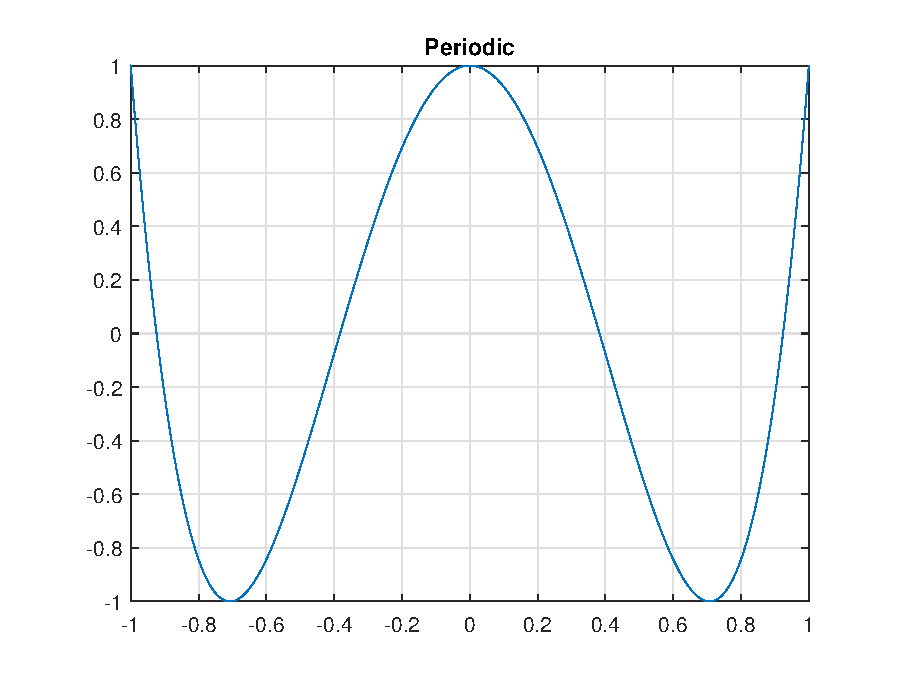
\includegraphics[height = 6cm]{Figures/Periodic}
			\end{figure}
		\end{enumerate}
	\end{problem}


\end{document}
